\begin{minipage}{0.63\textwidth}
    \parskip=1em
    \section*{セキュリティモジュール:3重安全装置}
    
    \uline{概要}:12個の丸い色分けされたボタンとギリシャ語のアルファベットの文字が付いたシャッター、有名な科学者の名前が書いております。
    
    \uline{解除方法}:連続する2つの鍵をそれぞれ開き、正しい4桁のコードを入力します。
\end{minipage}%
\hfill%
\begin{minipage}{0.33\textwidth}
    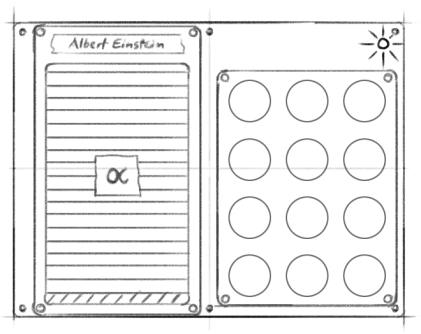
\includegraphics[width=\textwidth]{images/31.png}
    \vspace*{\fill}
\end{minipage}

\uline{A. 一つ目の鍵}:色分けされたボタンの正しい組み合わせを押します。\\
組み合わせは次のように決定されます。\\
\hspace*{1em}1. シャッターに見えるギリシャ文字、\\
\hspace*{1em}2. 科学者の名前。\\
次の表に可能な組み合わせを示します。\\
ボタンの数と色が正しければ、どのボタンを押してもかまいません。

\bgroup
\def\arraystretch{1.3}
\fontsize{9.5}{11}\selectfont
\begin{tabular}{c|cccccccc|}
\cline{2-9}
    &
    \multicolumn{8}{c|}{シャッターに付いているギリシャ文字} \\ \hline
\multicolumn{1}{|c|}{科学者} &
    \multicolumn{1}{c|}{\vphantom{\Huge A}\scalebox{2}{$\alpha$}} &
    \multicolumn{1}{c|}{\vphantom{\Huge A}\scalebox{2}{$\beta$}} &
    \multicolumn{1}{c|}{\vphantom{\Huge A}\scalebox{2}{$\gamma$}} &
    \multicolumn{1}{c|}{\vphantom{\Huge A}\scalebox{2}{$\delta$}} &
    \multicolumn{1}{c|}{\vphantom{\Huge A}\scalebox{2}{$\varepsilon$}} &
    \multicolumn{1}{c|}{\vphantom{\Huge A}\scalebox{2}{$\zeta$}} &
    \multicolumn{1}{c|}{\vphantom{\Huge A}\scalebox{2}{$\eta$}} &
    \multicolumn{1}{c|}{\vphantom{\Huge A}\scalebox{2}{$\theta$}} \\ \hline
\multicolumn{1}{|c|}{\begin{tabular}[c]{@{}c@{}}Albert Einstein\\ 1879-1955\end{tabular}} &
    \multicolumn{1}{c|}{\begin{tabular}[c]{@{}c@{}}1Y 2G\\ 1R\end{tabular}} &
    \multicolumn{1}{c|}{2Y 2G} &
    \multicolumn{1}{c|}{1G 3R} &
    \multicolumn{1}{c|}{3Y 1R} &
    \multicolumn{1}{c|}{4G} &
    \multicolumn{1}{c|}{4R} &
    \multicolumn{1}{c|}{4Y} &
    \begin{tabular}[c]{@{}c@{}}1Y 1G\\ 2R\end{tabular} \\ \hline
\multicolumn{1}{|c|}{\begin{tabular}[c]{@{}c@{}}Isaac Newtwon\\ 1643-1727\end{tabular}} &
    \multicolumn{1}{c|}{4G} &
    \multicolumn{1}{c|}{4R} &
    \multicolumn{1}{c|}{2Y 2R} &
    \multicolumn{1}{c|}{1G 3R} &
    \multicolumn{1}{c|}{2G 2R} &
    \multicolumn{1}{c|}{\begin{tabular}[c]{@{}c@{}}1Y 2G\\ 1R\end{tabular}} &
    \multicolumn{1}{c|}{3Y 1G} &
    3Y 1R \\ \hline
\multicolumn{1}{|c|}{\begin{tabular}[c]{@{}c@{}}Marie Curie\\ 1867-1934\end{tabular}} &
    \multicolumn{1}{c|}{2Y 2G} &
    \multicolumn{1}{c|}{1Y 3R} &
    \multicolumn{1}{c|}{\begin{tabular}[c]{@{}c@{}}2Y 1G\\ 1R\end{tabular}} &
    \multicolumn{1}{c|}{1Y 3G} &
    \multicolumn{1}{c|}{3Y 1R} &
    \multicolumn{1}{c|}{2G 2R} &
    \multicolumn{1}{c|}{4R} &
    3G 1R \\ \hline
\multicolumn{1}{|c|}{\begin{tabular}[c]{@{}c@{}}Louis Pasteur\\ 1822-1895\end{tabular}} &
    \multicolumn{1}{c|}{2Y 2R} &
    \multicolumn{1}{c|}{\begin{tabular}[c]{@{}c@{}}1Y 2G\\ 1R\end{tabular}} &
    \multicolumn{1}{c|}{4R} &
    \multicolumn{1}{c|}{3Y 1G} &
    \multicolumn{1}{c|}{1G 3R} &
    \multicolumn{1}{c|}{\begin{tabular}[c]{@{}c@{}}2Y 1G\\ 1R\end{tabular}} &
    \multicolumn{1}{c|}{2Y 2G} &
    4Y \\ \hline
\multicolumn{1}{|c|}{\begin{tabular}[c]{@{}c@{}}Nikola Tesla\\ 1856-1943\end{tabular}} &
    \multicolumn{1}{c|}{2G 2R} &
    \multicolumn{1}{c|}{\begin{tabular}[c]{@{}c@{}}2Y 1G\\ 1R\end{tabular}} &
    \multicolumn{1}{c|}{3Y 1R} &
    \multicolumn{1}{c|}{4Y} &
    \multicolumn{1}{c|}{1Y 3G} &
    \multicolumn{1}{c|}{\begin{tabular}[c]{@{}c@{}}1Y 1G\\ 2R\end{tabular}} &
    \multicolumn{1}{c|}{3G 1R} &
    4G \\ \hline
\multicolumn{1}{|c|}{\begin{tabular}[c]{@{}c@{}}Thomas Edison\\ 1847-1931\end{tabular}} &
    \multicolumn{1}{c|}{4R} &
    \multicolumn{1}{c|}{4Y} &
    \multicolumn{1}{c|}{4G} &
    \multicolumn{1}{c|}{1Y 3R} &
    \multicolumn{1}{c|}{2Y 2G} &
    \multicolumn{1}{c|}{3G 1R} &
    \multicolumn{1}{c|}{2Y 2R} &
    1G 3R \\ \hline
\multicolumn{1}{|c|}{\begin{tabular}[c]{@{}c@{}}Blasie Pascal\\ 1623-1662\end{tabular}} &
    \multicolumn{1}{c|}{1G 3R} &
    \multicolumn{1}{c|}{2G 2R} &
    \multicolumn{1}{c|}{\begin{tabular}[c]{@{}c@{}}1Y 1G\\ 2R\end{tabular}} &
    \multicolumn{1}{c|}{2Y 2R} &
    \multicolumn{1}{c|}{3Y 1G} &
    \multicolumn{1}{c|}{1Y 3R} &
    \multicolumn{1}{c|}{\begin{tabular}[c]{@{}c@{}}1Y 1G\\ 2R\end{tabular}} &
    1Y 3G \\ \hline
\multicolumn{1}{|c|}{\begin{tabular}[c]{@{}c@{}}Galileo Galilei\\ 1564-1642\end{tabular}} &
    \multicolumn{1}{c|}{3Y 1G} &
    \multicolumn{1}{c|}{2Y 2G} &
    \multicolumn{1}{c|}{1Y 3G} &
    \multicolumn{1}{c|}{4G} &
    \multicolumn{1}{c|}{\begin{tabular}[c]{@{}c@{}}2Y 1G\\ 1R\end{tabular}} &
    \multicolumn{1}{c|}{3Y 1R} &
    \multicolumn{1}{c|}{\begin{tabular}[c]{@{}c@{}}1Y 2G\\ 1R\end{tabular}} &
    1Y 3R \\ \hline
\end{tabular}
\egroup

\begin{center}
    Y -- 黄\qquad G -- 緑\qquad R -- 赤
\end{center}

例:1Y 2G 1Rの組み合わせの場合{、}次のボタンを押します。
\begin{center}
    黄色のボタン1つ{、}緑色のボタン2つ{、}赤色のボタン1つ。
\end{center}

\newpage

\uline{B. 二つ目の鍵}:ギリシャ文字が書かれた6つの四角いボタンのうち3つを押します。 正しい組み合わせは、次のように決定されます。\\
\hspace*{1em}1. 2番目のシャッター(6つの四角いボタンの下のドア)の色、\\
\hspace*{1em}2. 見えるギリシャ文字のセット。\\
以下の可能な組み合わせの1つだけが{、}爆弾モジュールの組み合わせと一致します。


\begin{center}
\def\makecell#1#2#3{\vphantom{\Huge A}\scalebox{1.5}{$\>{#1}\quad{#2}\quad{#3}\>$}}
\def\arraystretch{1.5}
\fontsize{10.5}{11}\selectfont
\begin{tabular}{c|cccc|}
\cline{2-5}
                            & \multicolumn{4}{c|}{可能な組み合わせ}                                            \\ \hline
\multicolumn{1}{|c|}{シャッターの色} & \multicolumn{1}{c|}{組み合わせ} & \multicolumn{1}{c|}{組み合わせ} & \multicolumn{1}{c|}{組み合わせ} & 組み合わせ \\ \hline
\multicolumn{1}{|c|}{青}  & 
\multicolumn{1}{c|}{\makecell{\alpha}{\delta}{\zeta}} & 
\multicolumn{1}{c|}{\makecell{\gamma}{\varepsilon}{\varkappa}} & 
\multicolumn{1}{c|}{\makecell{\beta}{\eta}{\psi}} & 
                    \makecell{\pi}{\mu}{\theta} \\ \hline
\multicolumn{1}{|c|}{灰色} & 
\multicolumn{1}{c|}{\makecell{\varrho}{\delta}{\varkappa}} & 
\multicolumn{1}{c|}{\makecell{\alpha}{\eta}{\zeta}} & 
\multicolumn{1}{c|}{\makecell{\iota}{\xi}{\lambda}} & 
                    \makecell{\psi}{\nu}{\mu} \\ \hline
\multicolumn{1}{|c|}{紫}  & 
\multicolumn{1}{c|}{\makecell{\tau}{\xi}{\beta}} & 
\multicolumn{1}{c|}{\makecell{\eta}{\iota}{\nu}} & 
\multicolumn{1}{c|}{\makecell{\delta}{\lambda}{\upsilon}} & 
                    \makecell{\varrho}{\omega}{\varepsilon} \\ \hline
\multicolumn{1}{|c|}{茶色} & 
\multicolumn{1}{c|}{\makecell{\sigma}{\gamma}{\varkappa}} & 
\multicolumn{1}{c|}{\makecell{\theta}{\zeta}{\pi}} & 
\multicolumn{1}{c|}{\makecell{\beta}{o}{\nu}} & 
                    \makecell{\omega}{\mu}{\alpha} \\ \hline
\multicolumn{1}{|c|}{橙色} & 
\multicolumn{1}{c|}{\makecell{\iota}{\nu}{o}} & 
\multicolumn{1}{c|}{\makecell{\lambda}{\gamma}{\sigma}} & 
\multicolumn{1}{c|}{\makecell{\chi}{\varepsilon}{\pi}} & 
                    \makecell{\psi}{\varrho}{\theta} \\ \hline
\end{tabular}
\end{center}

\uline{C. 4桁コード}:矢印を使用して数字を変更します。 正しいコードはその科学者が亡くなった年です。
